\documentclass[english]{article}
\usepackage{amsfonts}
\usepackage{dot2texi}
\usepackage[utf8]{inputenc}
%\usepackage{babel}
\usepackage[backend=bibtex, url=false]{biblatex}
\usepackage{hyperref}
\usepackage{mathtools}
\usepackage[printonlyused]{acronym}
\usepackage{minted}
%\usepackage{amsthm}
\usepackage{amsmath}
\usepackage{tikz}
\usepackage{graphicx}
\usepackage[linesnumbered, boxed]{algorithm2e}
\usepackage{amssymb}

\usetikzlibrary{shapes,arrows}

\hypersetup{
    colorlinks,
    citecolor=black,
    filecolor=black,
    linkcolor=black,
    urlcolor=black
}

\bibliography{library.bib}

% Add mathematical foo
\newcommand{\EI}{\operatorname{EI}}
\newcommand{\normal}{\mathcal{N}}
\newcommand{\x}{\mathbf{x}}
\newcommand{\E}{\mathbb{E}}
\newcommand{\M}{\mathcal{M}}
\newcommand{\X}{\mathcal{X}}
\DeclareMathOperator*{\argmin}{arg\,min}
\DeclareMathOperator*{\argmax}{arg\,max}


\begin{document}

%\title{Bayesian Optimization in Self-Referential Search Spaces}
%\author{Moritz Meier}

\begin{titlepage}
	\centering
	%\includegraphics[width=0.15\textwidth]{example-image-1x1}\par\vspace{1cm}
	{\scshape\LARGE Universität Osnabrück\par}
	\vspace{1cm}
	{\scshape\Large Master Thesis\par}
	\vspace{1.5cm}
	{\huge\bfseries Bayesian Optimization in Self-Referential Search Spaces\par}
	\vspace{2cm}
	{\Large\itshape Moritz Meier\par}
	\vfill
	First Supervisor:\par
	\textsc{Prof.~Dr.~Gordon Pipa}\par
  \vspace{1cm}
  Second Supervisor:\par
	\textsc{Prof.~Dr.~Frank Jäkel}\par
	\vfill

% Bottom of the page
	{\large \today\par}
\end{titlepage}



\begin{center}
\textbf{Declaration of Authorship}
\end{center}
I hereby certify that the work presented here is, to the best of my knowledge and belief, original and the result of my own investigations, except as acknowledged, and has not been submitted, either in part or whole, for a degree at this or any other university.


\noindent\begin{tabular}{ll}
&\\[8ex]
\makebox[2.5in]{\hrulefill} & \makebox[2.5in]{}\\
Signature & \\[8ex]% adds space between the two sets of signatures
\makebox[2.5in]{\hrulefill} & \makebox[2.5in]{}\\
City, Date & \
\end{tabular}


\newpage

\tableofcontents
\newpage

\section*{List of Acronyms}
\begin{acronym}
  \acro{AI}{artificial intelligence}
  \acro{BO}{Bayesian Optimization}
  \acro{BOA}{Bayesian optimization algorithm}
  \acro{BGO}{Bayesian global optimization}
  \acro{DAG}{directed acyclic graph}
  \acro{EGO}{efficient global optimization}
  \acro{GO}{global optimization}
  \acro{HPO}{hyperparameter optimization}
  \acro{IAF}{information acquisition function}
  \acro{ML}{machine learning}
  \acro{SMAC}{sequential model-based algorithm configuration}
  \acro{SMBO}{sequential model-based optimization}
  \acro{GPR}{Gaussian Process Regression}
\end{acronym}

\section{Introduction}
In past years the growing amount of collected data caused a increasing application of automated data processing in a wide range of areas streching from  science to industry.
The hight demand of experts with an understanding of computer programming and statistical methods causes many people from other fields to expand their skill set into machine learning methods. Other than more traditional parts of software engeneering, machine learning is still in the process of finding efficient workflow standarts. More and more data processing software libraries targeting different aspects of machine learning application are released. Especially the need for easy-to-use /out-of-the-box solution movend big software companies to develop big systems with features like integratet plotting, data-IO or even model sharing. The dataflow processing computation model turned out especially suited for data processing.

Figure \ref{ml-workflow} shows a simlified view on a machine learning workflow. First an algorithm selected, which is trained to obtain a model. The model is validated to measure generalization. This process is repeated for different algorithms, until a satisfying performance reached, or (probabily more frequent) a time limit is exceeded. This selection procedure, which is not considered as training in the previous overview, is the subject of research in this treatise.
The selection is usually seen as a two step process: from the range of aplicable machine learning algorithms select the most promising and in a second step select algorithm's configuration. While the former one is almost always done manually the automation of the second one is research object of the field of hyperparamter optimization.
The often multimodal, mostly unknown and sometimes discontinous nature of hyperparamter optimization problem leads many users to apply the easy to implement, exaustive and uninformed grid search or random search. The only source of information about the objective function, that can be embraced, is often the evaluation for some parameter setting of the objective function itself. Model-based global optimization methods try to harness this information by estimatating the objection function, allowing to make predictions for unknown points. In this way the number of function evaluations should be kept low (since this is the costly step), while the amount of information about the objective function, especially good performing areas, which is obtained in the process should be maximized.
In recent years Bayesian optimization as a method for hyperparameter optimization received some attention. A Bayesain model of the objective function, which essential means to have a distribution over function values, enabled to express the trade of between exploration and exploitation as a form of inference.
The problem of also automating the choice of the ML-algorithm is classified as \textit{automated machine learning}. The Combined Algorithm Selection and Hyperparameter optimization problem is also denoted by its acronym \textit{CASH} \cite{feurer_efficient_2015}. The configuration space is of cause different among different algorithms, such that the presence or relevance of a parameter can be dependent of the algorithm search. Algorithms like Tree-Parzen-Estimator and SMAC have been developt to deal with this condition.
Going a step further the parameter space can become even more complicated. If one considers for example multilayer perceptrons, where the number of layers needs to be determined before the number of neurons per layer can be chosen. In this case the number of model paramters can be of arbitray number. (put kernel example maybe here!)
This work proposes a formalism to state optimization problems by describing the structure of search spaces together, that range from simple one-dimensional strucutres to complicated infinte structures. The second contribution is an algorithm that extends known Bayesian optimization algorithm, such that self-referential search space description can be examined in an efficent manner.
(make my point clearer here!)
Section 2 discusses the probelm of global black-box optimization in general. Section 3 narrows the view point to hyperparamter optimization.
Section 4 shortly introduces Gaussian process regression, since they are from the Bayesian model in the algorithms.
Section 5 explains methods of Bayesian optimization.
Section 6 describes the search space description formalism.
Finally section 7 exmplains the tree Bayesian algorithm.
Section 8 give some comments to the implementation and show code examples.
In Section 9 the results of a row of experiments that apply the system to various differnt problems is presented.

Metaheuristics
Programm Configuration
Learning \& Optimizaion.

DACE - design and analysis of computer experiment

\begin{figure}
  \includegraphics[scale=0.7]{figures/ml-workflow.pdf}
  \caption{Simplified overview of a machine learning workflow.}
  \label{ml-workflow}
\end{figure}

Bayesian optimization is a Bayesion approach to global black-box optimization with an application in Hyperparameter optimization.

\section{Hyperparameter Optimization}
Optimization problems occur in a wide range of fields in various different forms. There are different fields that are solely concerned with optimization problems of one kind or another. \textit{Mathematical programming} is the subbrach of applied mathematics, that is concerned with optimization. Classes of problems are stated formally, ofter together with with additional eqaulity or inequality contraints. The solution (algorithm) comes usually with a formal proofs of convergence or accurracy bounds. The field of \textit{Metaheuristics}
on the other side is rather based on intuitions, metaphoric priniciples and validation by simulation. A metaheuristic can be defined as "a high-level problem-independent algorithmic framework that provides a set of guidelines or strategies to develop heuristic optimization algorithms". \cite{sorensen_history_2014} Due to generality in method and application of the field, a vast amount of algorithms that are tageted to global optimization, led to a confusing (almost litteral) \textit{zoo of metaheuristics}. Researches with sometimes minor mathematical background, adopted metaphors from other scientific fields to describe algorithms in unconentional terminology which obscurify the relations to more established methods. \cite{sorensen_metaheuristics-metaphor_2015}

\subsection{Distinctions}


\paragraph{local vs. global} Local optimization as opposed to global optimization just aim to find local minimas. A local algorithm can be the basis of a global algorithm, for example with local optimization from different starting points.

\paragraph{gradient based vs. derivative free}
An algorithm which makes use of the first derivative of the objective function is called gradient based or a first order method. Algorithms that make use of the second derivative are called second order method. Famous examples are Gradient descent or newton method.

\paragraph{heuristic strategies vs. Exect methods}
aka. stochastic vs deterministic

\paragraph{model-based vs. instance-based}
More sophisticated \ac{GO} algorithms can be devided into
a.k.a. - model-free or direct

\paragraph{population vs. single instance}
Population based methods remember multiple isntances.

\subsubsection*{single vs multiobjective}


\subsubsection*{stochastic objective function}







The use of stochastic processe in \ac{GO} for surrogate fitting is called \ac{BO}. This approach was first explored by Harold Kushner in 1964 \cite{kushner_new_1964}. In \cite{jones_efficient_1998} the surrogate is also called \textit{figure of merrit}.


\subsection{Global Black-Box Optimization}



\subsection{Bandit Problem}
exploration-exploitation tradeoff


\subsection{Active Learning \& Experimental design}
Active learning is a related method, that is applied for classification task with lots of unlabeld data which, which are expensive to label. It is very similar to BO in the way that promising unlabeld datapoint are selected by a model, which is adapted to every new label. Differences are tha labels are delivered by a human (called the \textit{oracle}) and that the samples come usually from a finite set (\textit{pool based sampling}) \cite{settles_active_2010}.

 - optimal experimental design
 - response surface model

\subsection{Hyperparameter Optimization}
In Bayesain statistics the term \textit{hyperparameter} referes to a parameter of the prior distribution. In \textit{hierarchical models} the prior distribution over the hyperparamters are called \textit{hyperpriors} respectively \cite[p.408]{bishop_neural_1995}. In \acf{ML} a hyperparameter is any parameter that needs to be assigned before the training of other parameters can begin. The \ac{ML} definition is adopted here. The selection procedure usually involves repetitive training of \ac{ML}-algorithm with various hyperparameter combinations and rating by some quality measure. This nesting gives rise to an alternative label for hyperparameters as \textit{outer loop} in contrast to \textit{inner loop} parameters that are selected by the \ac{ML}-algorithm itself. \acf{HPO} Other terms for \ac{HPO} are hyperarameter \textit{search} or \textit{tuning}.
Also \textit{model selection} means essentially the same thing, the focus is more on the selection criterions.
A key characteristic of \ac{HPO} problems is littel knowledge about the search space structure.  While \ac{ML}-algorithms are usually defined in a way that inner loop parameters can be optimized efficiently.
\paragraph{Long evaluation times}
\paragraph{Little knowledge} of the objective function
\paragraph{varying complexity} of search space ranging from simple homogenic cartesian search spaces to heterogenic graph shaped spaces.

\subsection{Machine Learning as Optimization}
Most \acf{ML} problems are expressable as optimization problems \cite{bennett_interplay_2006}. Training algorithms are (usually) derived by solving the minimization problem of some error or energy function or maximization of fittnes or utility function. From this perspective learning on the most general level can be stated as a global black-box optimization problem problem.
$$\x^* = \argmin_{\x \in \mathcal{X}} f(\x)$$
A best general solution of this problem does of cause not exists. Due to \textit{No Free Lunch} theorem for optimization, which roughly speaking states that the average performance of any algorithm across all possible optimizaion problems is identical. In other words efficient optimization without any assumptions or prior over the hypothesis space is impossible. Luckily in most cases the assumption can be made that points which are close in the input space are probabliy also close their performance. This requires a topology (structure) of the search space, which is naturally given for numerical inputs.

In his famous \textit{Statistical Learning Theory}, Vladimir Vapnik states the \textit{General Setting of the Learning Problem} as a minimization of the risk function \cite{vapnik_overview_1999}.
\begin{equation}
R(\alpha) = \int Q(z,\alpha)dP(z)
\label{risk}
\end{equation}
The risk $R$ takes the role of the objective function. $P$ is the true probability distribution over the data. The function $Q$, which is parametrized by $alpha$, measures the performance on a single data point $z$. The structure of $Q$ is left open and incorporates a possible model, algorithm or loss function. While this genral risk function is not as general as the name may suggest it still covers a majority of problems in machine learning. Since $P$ is usually unknown and represented by samples as the data, it is estimated by the more practical empirical risk function.
\begin{equation}
R_{emp}(\alpha) = \frac{1}{l} \sum_{i=1}^l Q(z_i,\alpha)
\label{empirical risk}
\end{equation}
Depending on the problem the function $Q$ takes different forms. For supervised learning, for example, a data point $z$ is a tuple of a dependent and an independent variable $(x,y)$. The task is to find a function $f$ that maps from $x$ to $y$. Eventually $Q$ can be written in terms of a lossfunction $L(y,f(x,\alpha))$.
To make it even more specific the function $f$ is actually the result of a learning algorithm $\mathcal{A}$, which can be seen as a functor mapping hyperparameter setting $\lambda$ and a traningg set $X_{train}$ into the hypothesis space. This leads to the definition of the hyperparamter problem as it is defined by Bergstra et al. in \cite{bergstra_random_2012}.
\begin{equation}
\lambda^{(*)} = \argmin_{\lambda \in \Lambda} \E_{\x \sim \mathcal{G}_\x}\big[\mathcal{L}\big(\x;\mathcal{A}_\lambda(X_{train})\big)\big]
\label{hypa_opt_1}
\end{equation}
Equation \ref{hypa_opt_1} is a special case of the risk function, with $Q = \mathcal{L}$ and $\alpha$ the fitted model. Note that $X_{train}$ is not requiered to be sampled form $G_x$, and thus covers learning problems where the data in training and application is different.
In order to avoid overfitting and estimate the generalization error, model selection technics are applied. In special cases measures which trade off number of parameter and sample size with the training loss (like BIC or AIC) can be applied. In most practical application however, having a separated training and validation set is most popular. The empirical risc version of the hyperparmeter optimization looks like this:
\begin{equation}
  \Psi(\lambda) = \sum_{x \in X_{val}} \mathcal{L}\big(x;\mathcal{A}_\lambda(X_{train})\big)
\end{equation}
Optimizing over the whole hyperparameter space is not possible in the general case. The search is thus limites to a finite subset $\{\lambda_1, \lambda_2, ... \} \subset \Lambda$
\begin{equation}
  \hat{\lambda} = \argmin_{\lambda \in \{\lambda_1, \lambda_2, ... \}} \Psi(\lambda)
\label{empirical hypa_opt_1}
\end{equation}

% risk with loss function
%\begin{equation}
%R(\alpha) = \int L(y,f(x,\alpha))dP(x,y)
%\end{equation}

\begin{enumerate}
  \item approximation by iterration
  \item approximation by limit data
  \item approximation by less crossvalidation
  \item randomness in training process -> stochastic objective function
\end{enumerate}

Even if one can only make a few or no assumptions about the structure of a hyperparamter search space, one has always the option to use estimations to gather information about the function faster.


\begin{quote}
Machine learning algorithms, however, have certain characteristics that distinguish them from other black-box optimization problems.  First, each function evaluation can require a variable amount of time:  training a small neural network with 10 hidden units will take less time than a bigger net-work with 1000 hidden units.  Even without considering duration, the advent of cloud computing makes it possible to quantify economically the cost of requiring large-memory machines for learning, changing the actual cost in dollars of an experiment with a different number of hidden units.
\end{quote}
Second, machine learning experiment EGO algorithm


\paragraph{Demands to a good HPO-Algorithm}
A non-exaustive list of general criteria for a good hyperparameter optimization algorithm. ???
\paragraph{parallelizabel}
\paragraph{interactive}
\paragraph{scalability}
\paragraph{Assumptions}
\paragraph{approximations}
 - early stopping
 - data subset
 \subsection*{computational costs}
 - space \& time
 - intelligent selection vs massive sampling tradeoff


\section{Gaussian Processes Regression}
Regression is the problem of estimating the relationship between an indendent random variable $X$ and a real-valued dependent random variable $Y$, by generalizing from examples. In frequentist settings one ususally defines a parametrized familiy of underlying functions. A point estimator is then applied to find the set of parameters that explains/predicts the data the best. In the famous maximum likelihood approach the conditional likelihood of the data $P(Y|X)$ is maximised over the model parameters. The semi-Bayesian maximum a posteriori approach additionally assumes a prior probability over the model-parameters and can e.g. deal with overfitting in a natural way. Finally in the fully Bayesian approach the estimates are distributions over parameters rather than single paramters settings. Gaussian process regression goes even a step further by having a non-parameteric model that grows with in complexity with the amount of data (Some authers prefere to call them inifinte-parametric models for that reason).

A GP (Gaussian process) is a (usually infinite) collection of random variables where any finite subset is multivariat normal distributed. These random variables can be indexed by $\mathbf{x} \in \mathbb{R}^n$, such that the GP can be seen as a distribution over functions $\mathbb{R}^n \rightarrow \mathbb{R}, x \mapsto f(\mathbf{x})$. This is written like:
$$f(\mathbf{x}) \sim \mathcal{GP}\big(m(\mathbf{x}), \kappa(\mathbf{x},\mathbf{x}')\big)$$
Where $m$ is the function of the expected value, and $\kappa$ the covariance function, which specifies the covariance of the dependet variable with respect to the independent variable:

$$\operatorname{cov}(f(\mathbf{x}),f(\mathbf{x}')) = \kappa(\mathbf{x},\mathbf{x}')$$

For comptational simplicity the prior mean is usually set to $m(\mathbf{x}) = \mathbf{0}$. In order to sample from the prior, $K_{**} = \kappa(X_*,X_*)$ one can use the multivariat normal distribution.
$$\mathbf{f_*} \sim \mathcal{N}(\mathbf{0}, K_{**})$$

Even though the model is a Gaussian process, the calculations can be done with mutivaraite Gaussian distributions and have a time complexity of only $O(N^3)$.

The trick to conduct the conditional distribution, wich is required for prediction, is to formulate the joint distribution over observed points and the sample points:

$$
\begin{bmatrix}
\ \mathbf{y}\ \\
\ \mathbf{f_*} \\
\end{bmatrix}
\sim \mathcal{N} \Bigg(\mathbf{0},
\begin{bmatrix}
K_y & K_* \\
\ K^{\top}_{*} & K_{**}  \\
\end{bmatrix}
\Bigg)
$$

Next condition on the sample points to end up with the following:

$$\overline{\mathbf{f_*}} = K_*^\top K_y^{-1}\mathbf{y}$$
$$cov(\mathbf{f_*}) = K_{**} - K_*^\top K_y^{-1} K_*$$

For interpolation (noise free prediction) case $K_y$ euqals $\kappa(X,X)$. For noisy prediction $K_y$ gets and additional noise term $\kappa(X,X) + \sigma_n^2$.

\begin{figure}

  \begin{minipage}{0.5\textwidth}
  \includegraphics[scale=0.3]{figures/prior_plot.pdf}
  \end{minipage}%
  \begin{minipage}{0.5\textwidth}
  \includegraphics[scale=0.3]{figures/posterior_no_noise.pdf}
  \end{minipage}%

  \begin{minipage}{0.5\textwidth}
  \includegraphics[scale=0.3]{figures/posterior_with_noise.pdf}
  \end{minipage}%
  \begin{minipage}{0.5\textwidth}
  \includegraphics[scale=0.3]{figures/posterior_exp.pdf}
  \end{minipage}%

  \caption{Upper Left: Three samples for a Gaussian process with zero mean, and RBF Kernel. Upper Right: Posterior for some sample points, without noise term. The blue area displays the margin of the variance. Lower left: posterior with noise term. Lower right: Posterior with noise term and exponential kernel.}

\end{figure}


The actual implementation of \ac{GPR} requires further knowledge about numeric properties which are not discussed here. A practical algortihm description involving Cholesky decomposition can be found in \cite[Algorithm 2.1]{rasmussen_gaussian_2006}.




\subsection{Kernels}
A quadratic matrix $K$ with $\mathbf{v}^\top \mathbf{v} \ge 0$ for all $\mathbf{v} \in \mathbb{R}^n$.

The \textbf{squared-exponential} kernel (SE), which is also called radial basis function kernel (RBF), has many desireble properties. For closer points the correlation tends towards one for while the correlation of farer points tends towards zero. This leads to very smooth function.

\begin{itemize}
  \item local kernel
  \item stationary kernel
\end{itemize}

\paragraph{Kernel Hyperparamters}
Parameters are optimized by optimizing the margnial likelihood ...

\paragraph{Kernel Combination}
Kernel combination properties. Maybe: Why do they work!



\section{Bayesian Optimization}
Bayesian optimization is model-based optimization with a Bayesian model. The
- mential pelikan stuff

\subsection{SMBO}
Sequential model-based optimization is a very general algorithmic pattern for global optimization with aquistion functions.

\begin{algorithm}[H]
\SetAlgoLined

$S \leftarrow \emptyset$\;
\Repeat{stop criterion reached}
{
  $\mathcal{M} \leftarrow$ fitModel($S$)\;
  $\x_{next} \leftarrow \argmax_{\x \in \X} \alpha(\x|\M)$\;
  $y \leftarrow f(x_{next})$\;
  $S \leftarrow S \cup \{(x,y)\}$\;
}
\caption{SMBO}
\end{algorithm}

The algorithm starts by initializing an empty set $S$ that is about store pairs $(x,y)$ of argument and result of the objective function (line 1). Loop is entered that iterates until a stopping criterium is reached. Such a criterium is usually a timeout, maximal number of iterations or sufficient performance of a configuration (line 2 \& 7). A curve/model is fittet through the pairs in $S$ (line 3). The model is used to conduct inference about unseen points of the objection. The aquisition function calculates a value that indicates how usefull/promising an evaluation of a point is. The point with the maximal aquisition value gets selected to be the next evaluation point (line 4). The next point gets evaluated(line 5). Add new pair to set $S$ (line 6).

\begin{figure}
  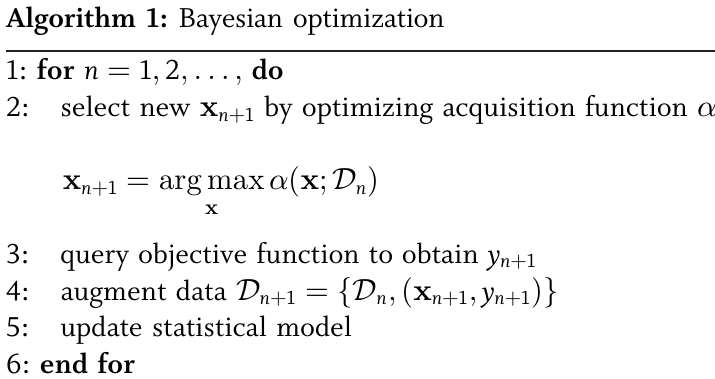
\includegraphics[width=1\textwidth]{figures/bayesian_optimization.png}
  \caption{Three steps in a Gaussian process based SMBO.}
  \label{bayesian optimization}
\end{figure}

\subsection{Aquisition Functions}

The role of the aquisition function is to quantify how profitable an evaluation of the objective function is for a point $\x$. The location of the best known value of the aquisition function is the next point that will be evaluate. It is a trade off between exploitation of less known regions and exploitation of promising areas. The function described in the following can all be brought into the form:

$$\alpha(\x) = \E_{y|\x}[U(\x,y)]$$

Where $U$ is an utility function. In experiemtal design $\alpha$ is therefore also known as the expected utility.
A very aquistion is used by the

$$\alpha_{UCB}(\x) \coloneqq \mu(\x) + \beta \cdot \sigma(\x) $$

\paragraph{Probability of Improvement}

(Kushner 1964)

$$
\alpha_{PI}(\x) \coloneqq \mathbb{P}[v>\tau] = \Phi\bigg(\frac{\mu(\x)-\tau}{\sigma(\x)}\bigg)
$$

With this definition

\paragraph{Expected Improvement}
Expected Improvement (EI) was first used by Mockus et al. in 1978 \cite{mockus_application_1978} in the context of noise free computer experiments. The first application to Bayesian optimization was done by Jones in 1998 \cite{jones_efficient_1998}, who called hist approach \textit{efficient bayesian optimization}(EGO). Since empirical studies have shown good results for EI (CITATION HERE) it has become widely adopted. The utility for EI is the so called improvment function.
$$\alpha_{\EI}(\x) \coloneqq \E_{y|\x}\big[(y - \tau)\mathbf{I}_{[y > \tau]}\big]$$
With $\tau$ beening a treshold that is usually chosen as the best observed performance of the objective function $y_{max}$. $\mathbf{I}$ denotes the indicator function that equals one if $y$ is bigger than the treshold and zero if it is smaller of equal. For a Gaussian model the EI can be witten in closed form:
$$ \alpha_{\EI}(\x) = \int\limits_{\mathbb{R}} \max(0, y-\tau)p(y|\x)dy$$
$$= (\mu(\x) - \tau) \cdot \Phi \bigg(\frac{\mu(\x)-\tau}{\sigma(\x)}\bigg) + \sigma \cdot \phi \bigg(\frac{\mu(\x)-\tau}{\sigma(\x)}\bigg)$$
$\phi$ is the standart normal PDF and $\Phi$ the standart normal CDF. $\mu$ and $\sigma$ are expected value and standart deviation of the model at point $\x$.
For a derivation of the closed form see appendix \ref{EI derivation}.

\paragraph{other aquisition functions}
Entropy search, Upper confidence bound

\subsection*{Aquisition optimization}
The use of a model and an aquisition function leads to a new non-convex optimization problem. Algorithms to find the maximum of the figure of merrit include global optimization technics uschas: DIRECT, L-BFGS-B, ...

\subsubsection*{Recommendation Strategy}
The need for a recommendation strategy arises for noisy objective functions. In the deterministic setting the maximal aquisition value becomes the recommendation for the next evaluation step. For non-det erministic aquisition function one needs to generate a sample from a distribution over aquisition values. Strategies like returning the maximum observed value or returning the optimal latent posterior mean can be encountered. Different objective function can require different strategies \cite{hoffman_modular_2014}.

\subsection{Noisy Objective Functions}
In machine lerning experiments the objective function can be noisy, if explicite randomness is used in the algorithm or when approximation of the real function are used.
\subsection{Conditional Parameters}

\paragraph{SMAC}

\paragraph{The Tree-Parzen Algorithm}
The Tree-Parzen Algorithm \cite{bergstra_algorithms_2011} is a Bayesian-Optimization algorithm for tree-structured parameter spaces.

\paragraph{Tree and Graph Kernels/Metrics}
...



\section{Search Space Construction}


\begin{table}
  \begin{tabular}{| l | l |}
    \hline
    name & definition \\
    \hline \hline
    objective function & function to be optimized \\
    search space &  domain of the objective function that is subject to the optimization\\
    program space & search space together with the objective function \\
    parameter space & search space \\
    expression & representation of a search space, comprising primitive parameters and \\
    grounded expression & expression where the cardinality of the extension equals one \\
    instance & grounded expression \\
    extension & set of all instances of an expression \\
    semantic equal & equal extension \\
    structural equal & ... \\
    computation graph & instance with graph structure \\
    computation tree & instance with tree structure \\
    parameter & unspecified value, that is subject to the optimization \\
    input & unspecified value, that is not subject to optimization \\
    output & return value / space of the output \\
    (computation) node & primitive node or application node \\
    operation & wrapper of a function, creates a computation node when called, input and outputs must be value \\
    combination & if evaluable: inputs and outputs can be computation graphs \\
    grammar & self-referential expression \\
    selection & ... \\
    projection & ... \\
    restriction & implicite selection via constraints \\
    domain & all possible values of a parameter ... \\
    parameter list & parameter family without named parameter \\
    parameter family - \\
    argument & value that is applied to a function / value of a parameter family \\
    crown & list of independent choices of an expression \\
    flat expression & expression without joined nodes \\
    \hline
  \end{tabular}
  \caption{Definitions}
  \label{definitions}

\end{table}



The majority of \ac{HPO} algorithms are designed for domains of the form $\mathbb{R}^n$.
The basic idea underlying the construction of parameter spaces is that variables do not need to possess a unique value assingment, but can rather have a set of or possible values. Instead of saying $x = 1$ one can say that $x$ equals ether one or two. Any other operations that Finally this set of computation graphes can be applied to a performance measure, expressing an optimization problem with instances of the computation graph set as possible solutions.

A search space is not a set but induces a unique set. The set of all instances that can be produced by a search space description $G$ is called the \textit{extension} of $G$ and expressed with a following apostrophe $G'$. While a unique extension can be assigned to every search space, an extension can be represented by multiple search spaces.

\subsection{Primitive Spaces}
The smallest unit of a search spaces is a primitive space. It is a one dimensional collection of possible instances of a parameter. Every search space is ether a primitive space of a combination of primitive spaces.

\paragraph{Categorical}
Categoriacal parameters have a finite unsorted domain of numerical or non-numerical values. This type is used for nominal scaled parameters like labels in a classification problem, basis-functions in linear regression or different activation functions in feedforward neural networks.

\paragraph{Continuous}
Continues parametes are bounded or unbounded intervals over the real numbers. This type would, for example, be used for a regularization parameter or the discount factor in Q-learning.

\paragraph{Discrete}
Values of a discrete parameters are numerical. The cardinality of a discrete parameter is finite or countable (if defined over an unbounded interval).
Other than categorical parameters, but similar to continous parameters, discrete parameters have a distance over their elements. If two elements are close, than the value of the objective fucntion is also assumed to be closed. This type is, for example, used as the number of layers in a neural network.

\subsection{Combinations}
Combinations take search spaces and return a combined search space. A combined search space is represented by an application node which posseses an operation and a domain field. Combined search spaces can be combined again in order to create strcutured search spaces. The operation field is assiged with combinator itself, while the domain is assigned with a parameter family.
In programming languages, when calling a function, the parameters are usually passed-by-name, passed-by-value or both. Mathematically this can be expressed by an indexed family. The passed-by-value arguemts are indexed by integers from $0$ to $n$ and the passde-by-name argumets are indexed by strings. A parameter family with two positional arguments $A,B$ and a key keyword argument $C$ with index $\gamma$ is written as:
$$\{A_0, B_1, C_\gamma\}$$

\paragraph{Joining}
Two search spaces $A$ and $B$ can be joined to form a new search space, which contains all instances of $A$ and $B$. In recemblence to the Backus–Naur form, the join combination can also be expressed through a pipe symbol.
$$ \operatorname{join}(A, B) = A\ |\ B $$
The join is related to the set union, in that the extension of the join of two search spaces is the union of the extensions of these search spaces: $(A\ |\ B)' = A' \cup B'$. The only difference is that a join remembers the spaces it was constructed from.

\paragraph{Product}
The product lines up multiple search spaces to form a sequence of search spaces. It expressed by the $\operatorname{prod}$. If evaluated the product is evaluated it returns a parameter family.
$$\operatorname{eval}(\operatorname{prod}(A, B, C)) = \{A_0, B_1, C_2\}$$
The extension of a product of two spaces is the cartesian product of the extension of these two spaces: $\operatorname{prod}(A,B)' = A' \times B'$. In constrast to the cartesian product, the product of search spaces is associative.  In this way no nested structures can be constucted with the product alone. If evaluated the product returns a parameter family. Under the hood
The cartesian product of two parameter families is defined as follows. If all indices are integers the product is a usual cartesian product. The length of the first family is added to all indices of the second tuples.
$$\{A_0, B_1\} \times \{C_0, D_1\} = \{A_0, B_1, C_2, D_3\}$$
Non-integer indices are simply copied to the resulting family.
$$\{A_0,\ B_\beta\} \times \{C_0,\ D_\delta\} = \{A_0,\ C_1, B_\beta,\ D_\delta\}$$
The prodcut is undefined if two non-positional parameters share the same key.

\paragraph{Quoting}
In some cases it is required to hand an unevaluated computation tree to an operation. In reseblence to the correstponding operator in the Lisp programming, this is expressed by the $\operatorname{quote}$ operation. It is simply a wrapper for a computation tree, that returns the computation tree if evaluated.

\paragraph{Projection}
Elements can by selected from parameter family through the projection $\pi$.
$$\pi_1(\{A_0, B_1, C_\gamma\}) = B$$
The correstponding operation is $project$.

\paragraph{Rename}
Items of a parameter family can be renamed. In resemblence to relational algebra the greek letter $\rho$ is used to refer to the rename.
$$\rho_{1/a}(\{A_{0}, B_{1}\}) = \{A_{0}, B_{a}\}$$
The corresponding operation is $rename$. The rename can be used in to change the order.

\paragraph{Function Application}
Any function can be integrated into the system by converting it to an operation with the "op" function. If a parameter is applied to an operation an apply node is created that simply represents the application of the underlying function to the arguments. An alternative way to express application with is with the @ symbol.
$$f(A) = f\ @\ A$$

Parameters can also be applied to joined spaces. This is equivalent the join of the correstponding function application node.
$$(f\ |\ g)(A) = f(A)\ |\ g(A)$$

With function application it finally becomes possible to express \textit{dependendencies} between parameters.
$$f(B)\ |\ g(C)$$
If $B \neq C$ then the function $f$ and $g$ have different parameter domains. The choice of the parameter is dependent on previous choice of the function.  The structure of the search space is not a vector any more but becomes a tree. (put this further down)

\paragraph{Recursion}
With recursion it is possibel to express self-referential search spaces. This is done by introducting the insertion operator "$<<$" which distingiushes itself from any other previous functions by its capability to change an expression, as opposed to just combining expressions to a new one. The insertion appends into the parameter family of a node. In this manner expressions that have $G$ as a substructure can be inserted into $G$. Consider the following construction of $G$:
$$G \leftarrow join(A)$$
$$ G  \ll f(G, G)$$
In the first line $G$ is initialized be an empty join node. In the second line an

The extension of an expression is defined as the  :

$$ A' = \{\mathbb{N},\ f(\mathbb{N}, \mathbb{N}),\ f(\mathbb{N}, f(\mathbb{N}, \mathbb{N})), ... \}$$

In this way the function nesting can become arbitrary deep. The search space becomes an infinite tree, but the instances stay finite trees.

\paragraph{Selection}
In a generative grammar, sentences can be generated by a successive rule application. A sample from a search space can be generated by successively selecting from the joined nodes.
$$X \leftarrow (A\ |\ B)\ |\ (C\ |\ D)$$
$$\sigma_1(X) = (C\ |\ D)$$

To select from more complicated search space the notion of the choice shape needs to be introduced. Consider the recursive function tree definition of $G$:

$$ G \leftarrow \operatorname{join()}$$
$$ G \ll (f(G,G)\ |\ A)$$

In the first step Variable $G$ gets initialized with an empty join-node. In the second step a function $f$ with $G$ in both arguments and primitive search space $A$ are inserted into the join-node. The join node $G$ has two options, that can be chosen by a selection function. If we select the first option $f(G,G)$, we are faced with two times two choice options and need to select from four options in the next step. Note that the extension of a selected subspace is a subset of the extension of the superspace.

$$ f(A,A)' \subset f(G,G)' \subset G' $$

 The selection shape is a tuple that indicates the selection range of a search space. The calculation of the selection shape requires a graph traversion.

$$\operatorname{shape}\big(G\big) = (2,)$$
$$\operatorname{shape}\big(f(G,G)\big) = (2,2)$$
$$\operatorname{shape}\big(f(G,f(G,G))\big) = (2,2,2)$$

The length of the shapes tells the number of choices that can be made at the same time. The items of the choice space are the number of options per choice.

\begin{figure}

  \begin{dot2tex}[tikz,options=-t math]
    digraph G {

    node [shape=box]

    b [label="f(G,G)"]
    c [label="f(A,A)"]
    d [label="f(A,f(G,G))"]
    e [label="f(f(G,G),A)"]
    f [label="f(f(G,G),f(G,G))"]

    G -> A [label="0"]
    G -> b [label="1"]
    b -> c [label="0,0", lblstyle="left=1.1cm"]
    b -> d [label="0,1"]
    b -> e [label="1,0"]
    b -> f [label="1,1"]

    }
  \end{dot2tex}


  \caption{Three selection levels of search space $G$. }
  \label{levels}
\end{figure}

Reffering to the

\paragraph{Expression Equality}
Context free grammars can produce identical strings with a different sequence of production application. The same is true for parameter space definitions.
If a function to measure the equality of two expressions is added to the system, the search space obtains the structure of a directed acyclic graph.
Two expressions can have the same meaning even if the representations are not equal. So far this is

\paragraph{Constants \& Variables}
So far it is only possible to express search spaces over function trees.
A value that is computed once can only be used in a single other function call. With the introduction of \textit{constants} it is possible to remember the output of a computation tree evaluation. Implementationwise the constant is a wrapper around a search space, that remembers the first chosen value of that search space.
Constants allow to express structures beyond the capabilities of a context free grammars. For example a search space over matricies with arbitray size:

Variables are like constants, with additional ability to change value in the computation process. The elements of the search space obtain a cylic graph structures.
Both constants and variables are not integrated into the system and will not be discussed further.

\subsection{Simplification}
Simplification of the search space expression can improve comprehensibility for humans, but can also improve performance of optimization algorithms working with it. The other use of simplification is the transformation of instance expressions into a normal form, in order to detect equality of expressions.
Simplification can be realized by using methods used by term rewriting systems. In our case we can directly work on computation trees/graphs,  simplification is a tree/graph transformation. Operations can be supplemented with properties, which indicate legal transformations to the system.

\paragraph{commutative} Commutativity as known from binary operators indicates a symmetric realation. The order in which the arguments are applied is irrelevant. This notion can be extended to multvariate functions. The system can arbitrarily change the argument order. To bring an application of a commutative function into normal form, the parameters are sorted in alphabetical order of its serialization.

\paragraph{associative} For three or more binary associative operators in a row the application order is irrelevant. Computation trees are invariant under tree rotation if the two involved nodes are in a parent-child relationship and the operations of the node are identic and associative. For associative nodes left-to-right application conforms to the normal-form.

\paragraph{variadic}
In programming languages a variadic function is a function, that has a variable arity. Here the definition is stricter and requieres the function to be defined on an arbitrary arity ($f(),\ f(x),\ f(x_1,x_2),\ f(x_1,x_2,...,x_n)$).  The property also implies that arguments of a left-to-right applications of a node with equal operation can be merged into the parent node. An example of this is is given with the sum operation, depicted in Figure \ref{as/var transform}.

\begin{figure}

\begin{minipage}[b]{0.35\textwidth}
\caption{Two parsings of $a+b+c$. The left computation graph shows a usual left-to-right parsing, also written as sum(sum(a,b),c). With the as/var properties it can be simplified to the right computation graph sum(a,b,c).}
\label{as/var transform}
\end{minipage}%
\hfill%
\begin{minipage}[b]{0.3\textwidth}
\centering
\includegraphics[scale=0.3]{figures/sum_not_simplified.pdf}

% \label{Text}
\end{minipage}%
\hfill%
\begin{minipage}[b]{0.3\textwidth}
\centering
\includegraphics[scale=0.3]{figures/sum_simplified.pdf}
\end{minipage}%
\end{figure}

If the operation is also associative, child nodes with equal-operation can be merged into the parent node from any position (Table \ref{funcprops} row: ac/var).

\paragraph{Distributivity} is a property between two functions that is known from arithmetic addition and multiplication. In regard to search space expressions, function application is left and right distributive to joining.

$$f(A|B) = f(A)\ |\ f(B)$$
$$(f|g)\ @\ A = f(A)\ |\ g(A)$$
$$(f|g)\ @\ (A|B) = f(A)\ |\ f(B)\ |\ g(A)\ |\ g(B)$$

\paragraph{other proerties}
Idempotence can have two different meanings.

If a function is variadic, associative, commutative and binary idempotent it follows that any multiply occuring argument can be deleted. Proof:

$$f(\alpha_1, \mathbf{x}, \alpha_2, \mathbf{x}, \alpha_3) \stackrel{com}{=}
f(\mathbf{x},\mathbf{x}, \alpha_1, \alpha_2, \alpha_3) \stackrel{as/var}{=}
f(f(\mathbf{x},\mathbf{x}), f(\alpha_1, \alpha_2, \alpha_3)) \stackrel{bid_1}{=}$$
$$f(\mathbf{x}, f(\alpha_1, \alpha_2, \alpha_3)) \stackrel{as/var}{=}
f(\mathbf{x}, \alpha_1, \alpha_2, \alpha_3)$$

This is for example the case for the join, which plays


\begin{table}
\centering
\begin{tabular}{c | c | l}
abbr & property name & definition \\
\hline
as               & associative        & $f(f(x,y),z) = f(x,f(y,z))$ \\
com              & commutative        & $f(x,y)=f(y,x)$ \\
ldis             & left distributive  & $f(x,g(y,z))=g(f(x,y),g(x,z))$ \\
rdis             & right distributive & $f(g(x,y),z)=g(f(x,z),g(y,z))$ \\
id               & identity           & $f(x) = x$ \\
uid              & unary idempotent   & $f(f(x)) = f(x)$ \\
bid$_{\text{1}}$ & binary idempotent  & $f(x,x) = x$ \\
bid$_{\text{2}}$ & \multicolumn{1}{|c|}{$-$} & $f(x,x) = f(x)$ \\
var              & variadic           & $f(f(x,y),z) = f(x,y,z)$\\
as/var           & \multicolumn{1}{|c|}{$-$} & $f(x,f(y,z)) = f(x,y,z)$ \\
\end{tabular}
\caption{Overview of function/combination properties}
\label{funcprops}
\end{table}


\subsection{Structure of Search Spaces}
The range of available combinations induces the search space structure and allows for different kinds of value structures. The structure of the search space again, conditions the class of optimizers that is applicable.
With no combinations and only the primitive spaces at hand, the search space must be one dimensional and the value structure a single value.
The product allows for vectors of primitives, the search space becomes multidimensional. Remember that the product is associative, which forbids
With the join operation it is possible to construct hierachical trees of choices. The structure of the values however, remains untouched.
Adding function application changes the value structure to a tree, the search space structure remains.
Only primitives, product and function application together, (labeld $PA$ in Figure \ref{space_structure}) forms the space that contains only flat structures. Adding the join combination to $PA$ forms $JPA$ and requieres algorithms with handling of conditional parameters.
With constants the structure of the describable structure is extended to a DAG and is called a \textit{computation graph}.


\begin{figure}
\includegraphics[scale=0.5]{figures/search_space_hierachy.pdf}

  \caption{The leftmost node represents a system with only primitive spaces. Following the edges from left to right, new operations are added. The field of a node holds the following information from top to bottom: initials of available operations, structure of search space and structure of resulting values. Constants and variables are not depicted.}
  \label{space_structure}
\end{figure}


\section{Optimization of Self-Referential Seach Space}

\subsection{}
Convential Bayesain optimization algorithms are only suitable for falt multidimesnional search spaces or search spaces containing conditional parameters (SMAC and TreeParzen). The specification language described in the previous chapters however allows for search spaces with an arbitrary amount of parameters. The following algorithm allows to employ any Bayesian optimization model for flat parameter spaces to be applied to recursive parameter spaces.

The basic idea of the algorihm is to select subspaces from the search space as long as no joined node is presend in the tree any more. The resulting search space has only function applications and primitives and is therefore flat. On this subspace a flat optimizer can be applied.

The algorihm creates a tree where every node represents an expansion of the previous expression. A working variable $W$ is initialized with the root node associated to the original search space $G$. If $G$ has join nodes, a full selection $G^*$ is chosen from $G$ due to some selection criterion. If $G^*$ has not been explored, a node is created. The node for $G^*$ is assigned to $W$. This steps are repreated until $W$ contains no join nodes any more. The resulting search space flat, a conventional \ac{BOA} is applied to select the next evaluation point from this search space. Since the selection criterion for a subspace makes use of the best aquisition value of the subspace's child nodes, each nodes keeps track of this value. After the chosen instance has been evaluated the results gets stored to the leaf node. The aquisition values have changed and need to be recalculated. The maximal aquisition value get propagated down through the meta tree as long as it is the best value in this subset. If the newly evaluated point hat the best observed performance, the aquisition values of all subtrees have to be recalculated.



\begin{algorithm}[H]
\SetAlgoLined
initialize Root with G\;
best\_value $\leftarrow$ $\infty$\;
\For{i $\leftarrow$  0 \KwTo n}{
  W $\leftarrow$ Root\;
  \While{W is not flat}{
    W $\leftarrow$ select(W, $crit$)\;
    \If{Next = null}{
      W $\leftarrow$ new node\;
    }
  }
  p = next(W)\;
  result = compute(p)\;
  W.protocol.append(p, result)\;
  \eIf{result $<$ best\_result}{
    best\_result = result\;
    update all\;
  }{
    update W\;
    down propagate best aquisition\;
  }
}


\caption{Bayesian Optimization for trees}

\end{algorithm}
%
% \While{not flat(W.search_space) }{asd}
\subsection*{selection criteria from subexpression}
In two cases the subexpression selection is striaght forward: If on choice has been explored, an expansion can simply be chosen by random. If all choices are have at least been explored twice, the subexpression with the highest aquisition value would ne chosen. Any case in between with explored and unexplored choices can be chosen by different criteria.
In the simplest approach a fix value, which servers as a default aquisition, would be assigned to any unexplored node. High default aquisitions would benefit exploration of unknown structures, for self-referential expressions this leads to a faster exploration of bigger structures. Lower values would rather encourage exploration of varaints of known structures.
A more sophisticated approch is to apply \ac{GPR} on every selection level as well.


\subsection{Extention to DAG-structured Search Spaces}
Some search spaces can be restricted by introducing an function, that detect if two search spaces share the same extension.
Identifying equivalent function trees with computer algebra systems.

\subsection{Parallelization}
A sequential Bayesian Optimization Algorithm can be extended to parrallel Algorithm with one simple trick. If an evaluation point is chosen, instead of waiting for the actual result, the expeced value estimate, which is easilz exessible with the Gaussian model, is inserted as a placeholder. The selection process is initiated again and will chose another point since the variance of the former point is zero. One the computation is complete the placeholder value is substituted by the real value. In this way objective function evaluations can be parralelized, while parameter selection keeps sequential.


\subsection{Integration with Manual Search}
Manual guidance before and during the optimization process.

\subsubsection*{Prior Information}
In machine learning preknowledge about the learning task can be consindered as choice and distribution over the hypothesis space. This is determined rather indirect by the choice of the \ac{ML}-algorithm and its hyperparameters (or distribution over hyperparameters) or in Bayesian method directly expressed via prior probabilities. Since gaussian processes regession is used here, the choice of the kernel
Prior infotmation can for example be an actual probabilistic prior over the search space. For random sampling this probability can just be used as the sampling probability. For model-based methods, which have no direct sampling, this probability can be interpreted as \textit{probability of improvement} or (more plausible) as \textit{probability of optimum}.

\subsubsection*{Search Hints}
A concept I labeled \textit{search hints} is a way to express external knowledge about the search space. I contranst to regular prior knowledge search hits can also be injected into search process on the fly. Intuitively a search hint just denotes good region to search. And once again it is not obvious how to translate this human instructions into the search process.
The easier part is to construct a probability distribution only from hints. If a hint is interpreted as a sample from the space of the probability of optimum then distribution estimation methods like Parzen-Window can be used. If one takes a squard exponential kernel, a hint translates to good region. To indicate better regions one would need to give multiple of samples from the same region, which is unfavourable. To solve this one could give weighted hints. Once again there are different ways to do this.
First one could assign the probability of optimium directly to a region. This however is hard to conceptualize for users and requires not to violate the normalization property (sum of hints must not excede one).
A second way is to allow values between zero and one, fit a curve, and normlize aferwards to get a probability of optimum. Which is much better, because a value of zero keeps the interpretation of zero probability and one get the interpretation of maximum probability. If one allows arbitrary big values for hints the down scaling of former hints could become easier. If one allows also negative values, and includes adding the absolute value of the smalles negative value to all hints, upscaling of former hints would become possible. In both extensions however one looses the interpretation of one and zero.
The third method interpretes hints as a modification of an already existing model.
In an active learning setting point hints can be handeled without an model modification, by simply forcing this hints into the processing queue.

intuitive way to do this is ascribing an increase in probability to positive hints and and decrease in probability to negative hints.

\paragraph{Credebility and Authority}
The \textit{credebility factor} or \textit{authority factor} is a way to ...

\subsection{Objective Function Approximation}


\section{Implementation}
The formalizm has been realized as a package for the Python programming language.

\subsection{Example: Minimum of two function}

\begin{minted}{python}
from baumschule import *

# declares the objective fucntion
@operation
def f(x, y):
    return x**2 + y**2

# declare parameter search space
search_space = f(
  x = R[-10:10],
  y = R[-10:10],
)

# minimize function wit 100 iterations
opti_obj = minimize(search_space, max_iter=100)
opti_obj.run()

\end{minted}

\subsection{Example: Kernel Grammar}

\begin{minted}{python}
import numpy as np
import GPy
from baumschule import *

# Bayesian information criterion of a GPy model
def bic(model):
    return -2 * model.log_likelihood() + np.log(len(model.X)) * model.size

kernel_dict = {
    'RBF' : GPy.kern.RBF,
    'EXP' : GPy.kern.Exponential,
    'BIAS': GPy.kern.Bias,
    'LINEAR' : GPy.kern.Linear,
}

# construct search space
K = convert(set(kernel_dict.keys()))
K.symbol = 'K'
K = op(kernel_dict.get)(K)(1)
G = join()
G << (K+G | K*G | K)
G = simplify(G)

# load data
data = load('01-airline.mat')
x_train = data['X']
y_train = data['y']

# define objective function
def objective(kernel):
    m = GPy.models.GPRegression(x_train, y_train, kernel)
    m.optimize()
    return bic(m)

# create and run optimization
opt_obj = minimize_func(objective, G, max_iter=100)
opt_obj.run()

\end{minted}


\subsection{Example: Multilayer Perceptron, with variable layers}
The ...


\begin{minted}{python}
from baumschule import *
from sklearn.neural_network import MLPClassifier
from sklearn.datasets import fetch_mldata
from sklearn.model_selection import train_test_split

mnist = fetch_mldata('MNIST original', data_home='~/data/baumschule')

X_train, X_test, y_train, y_test = train_test_split(
     mnist.data, mnist.target, test_size=0.4)

@operation
def train_and_validate(model):
    model.fit(X_train, y_train)
    score = model.score(X_test, y_test)
    error = -1 * score + 1
    return error

# define grammar for network layers:
# abitrary length tuple, with integrers between 1 and 100
nn = N[:100]
layers = join()
layers << (prod(nn, layers) | nn)
layers = tuple_op(layers) # converts parameter family to tuple
layers = simplify(layers) # merges the join nodes

# set parameters of classifier
parameters = convert({
    'hidden_layer_sizes' : layers,
    'activation' : {'identity', 'logistic', 'tanh', 'relu'},
    'learning_rate' :  {'constant', 'invscaling', 'adaptive'},
})

# apply paramters to classifier and model to validation routine
model_space = op(MLPClassifier)(parameters)
search_space = train_and_validate(model_space)

# run optimization and save results
min_obj = minimize(search_space, max_iter=100)
min_obj.run()
min_obj.observers['standard'].to_csv('mnist_mlp.csv')

\end{minted}

\begin{figure}
  \includegraphics[scale=0.6]{figures/mlp_search_space.pdf}
  \caption{Visualization produced by the "to\_dot" function, showing the search space of the multilayer perceptron. Red nodes are primitive, blue nodes are application, yellow means combination.}
  \label{mlp_search_space}
\end{figure}


\section{Experiments}
\subsection{Gaussian Process Regression}
\subsubsection{Kernel Combination Optimization}
\subsubsection{Kernel Parameter and Kernel Combination Optimization}
\subsection{Elastic Net Linear Regression}
\subsection{Feat-Forward Networks}
\subsection{Self Optimization}

\section{Conclusion \& Outlook}

\begin{enumerate}
  \item{Connection to Functional Programming}
  \item{Connection to Constraint Satisfaction Problems}
  \item{Connection to Probabilistic Programming}
  \item{Connection to Reinforcement Learning}
  \item{Integration with Workflow-Managers}
\end{enumerate}



\appendix

\section{Derivation of Expected Improvement}
\label{EI derivation}

$$\alpha_{\EI}(\x) := \mathbb{E}_{y|\x}[max(y-\tau, 0)]\ $$

$$= \int\limits_{\tau}^{\infty}(x-\tau)dp(y|\x) = \int\limits_{\tau}^{\infty}(x-\tau)\mathcal{N}(y;\mu,\sigma)dy$$

$$ = \frac{1}{\sigma\sqrt{2\pi}} \int\limits_{\tau}^{\infty}(y-\tau)e^{-\frac{1}{2}\big(\frac{y-\mu}{\sigma}\big)^2}dy =
\frac{1}{\sqrt{2\pi}} \int\limits_{(\tau-\mu)/\sigma}^{\infty}(u\sigma+\mu-\tau)e^{-\frac{1}{2}u^2}du$$

$$=\frac{1}{\sqrt{2\pi}}\bigg((\mu-\tau) \mkern-12mu \int\limits_{(\tau-\mu)/\sigma}^{\infty} \mkern-10mu e^{-\frac{1}{2}u^2}du + \sigma \mkern-12mu \int\limits_{(\tau-\mu)/\sigma}^{\infty} \mkern-10mu u e^{-\frac{1}{2}u^2}du \bigg)$$

$$=(\mu-\tau)\bigg|\ \Phi(u)\ \bigg|_{(\tau-\mu)/\sigma}^{\infty} \mkern-6mu + \ \ \ \sigma\bigg|-\frac{1}{\sqrt{2\pi}}e^{-\frac{1}{2}u^2}\bigg|_{(\tau-\mu)/\sigma}^{\infty}$$

$$=(\mu-\tau)\bigg(1-\Phi\bigg(\frac{\tau-\mu}{\sigma}\bigg)\bigg) + \sigma \cdot \phi \bigg(\frac{\tau-\mu}{\sigma}\bigg)$$

$$ = (\mu - \tau) \cdot \Phi \bigg(\frac{\mu-\tau}{\sigma}\bigg) + \sigma \cdot \phi \bigg(\frac{\mu-\tau}{\sigma}\bigg)$$

\section{Formal descriptions}
Join and prod over parameter-lists form an idempotent semiring:

$(A, \cup)$ is a idempotent commutative monoid (or join-semilatice with zero) with identity element $\emptyset$:
$$(a \cup b) \cup c = a \cup (b \cup c)$$
$$\emptyset \cup a = a \cup \emptyset = a$$
$$a \cup b = b \cup a$$
$$a \cup a = a$$

$(A, \times)$ is a commutative monoid with identity element $[\ ]$:
$$(a \times b) \times c = a \times (b \times c)$$
$$[\ ] \cup a = a \cup [\ ] = a$$

Product left and right distributes over join:
$$a\times(b \cup c) = (a\times b) \cup (a\times c)$$
$$(a \cup b)\times c = (a\times c) \cup (b\times c)$$

Product by $\emptyset$ annihilates $A$:
$$\emptyset \times a = a \times \emptyset = \emptyset$$



\printbibliography


\end{document}
